\documentclass[a4paper,12pt]{article}
\usepackage[utf8]{inputenc}
\usepackage[T1]{fontenc}
\usepackage[english]{babel}
\usepackage{amsmath}
\usepackage{booktabs}
\usepackage{geometry}
\usepackage{graphicx}
\usepackage{caption}
\usepackage{setspace}
\usepackage{hyperref}

\geometry{margin=1in}
\setstretch{1.2}

\hypersetup{
    colorlinks=true,
    linkcolor=blue,
    urlcolor=blue,
    citecolor=blue
}

\title{Event Study on Food Prices \\ \large Difference-in-Differences Analysis}
\author{Tim Birkert}
\date{\today}

\begin{document}

\maketitle

\section*{1. Introduction}

This report presents the results of an event study analyzing the impact of a fictitious treatment on average food prices. Using a Difference-in-Differences (DiD) approach with fixed effects for country and year, we estimate how prices evolved over time relative to the treatment event.

The dependent variable is the logarithm of the average price. Standard errors are clustered at the country level to account for intra-group correlation.

\vspace{1em}

\section*{2. Model Specification}

The estimated model takes the form:

\[
\log(\text{Average\_price}_{it}) = \sum_{k=-20}^{15} \beta_k \cdot \mathbf{1}(\text{year\_diff}_{it} = k) + \alpha_i + \lambda_t + \epsilon_{it}
\]

where:
\begin{itemize}
    \item $\mathbf{1}(\text{year\_diff}_{it} = k)$ are indicator variables for years relative to treatment ($k = -20, \ldots, 15$),
    \item $\alpha_i$ are country fixed effects,
    \item $\lambda_t$ are year fixed effects,
    \item $\epsilon_{it}$ is an error term clustered at the country level.
\end{itemize}

\vspace{1em}
\newpage

\section*{3. Results}

\begin{table}[ht]
\centering
\caption{Event Study Coefficients: Effects of Treatment Over Time}
\small
\begin{tabular}{lrrrr}
\toprule
Year Relative to Treatment & Estimate & Std. Error & t value & $p$-value \\
\midrule
-20 & -0.247 & 0.076 & -3.25 & 0.0022 ** \\
-19 & -0.212 & 0.061 & -3.46 & 0.0012 ** \\
-18 & -0.202 & 0.051 & -3.96 & 0.0003 *** \\
-17 & -0.188 & 0.045 & -4.15 & 0.0002 *** \\
-16 & -0.159 & 0.042 & -3.81 & 0.0004 *** \\
-15 & -0.143 & 0.040 & -3.59 & 0.0008 *** \\
-14 & -0.134 & 0.038 & -3.56 & 0.0009 *** \\
-13 & -0.088 & 0.035 & -2.50 & 0.0164 * \\
-12 & -0.082 & 0.032 & -2.56 & 0.0140 * \\
\vdots & \vdots & \vdots & \vdots & \vdots \\
6 & -0.057 & 0.026 & -2.16 & 0.0359 * \\
7 & -0.066 & 0.031 & -2.12 & 0.0398 * \\
8 & -0.073 & 0.036 & -2.07 & 0.0448 * \\
9 & -0.083 & 0.040 & -2.09 & 0.0424 * \\
10 & -0.091 & 0.044 & -2.08 & 0.0430 * \\
\bottomrule
\multicolumn{5}{l}{\footnotesize{Significance codes: *** $p<0.001$, ** $p<0.01$, * $p<0.05$}}
\end{tabular}
\label{tab:eventstudy_results}
\end{table}

\vspace{1em}

Model diagnostics:
\begin{itemize}
    \item Observations: 1,101
    \item Countries (Fixed Effects): 45
    \item Years (Fixed Effects): 26
    \item RMSE: 0.150
    \item Adjusted $R^2$: 0.610
    \item Within $R^2$: 0.020
\end{itemize}

\vspace{1em}
\newpage

\section*{4. Event Study Plot}

\begin{figure}[ht]
\centering
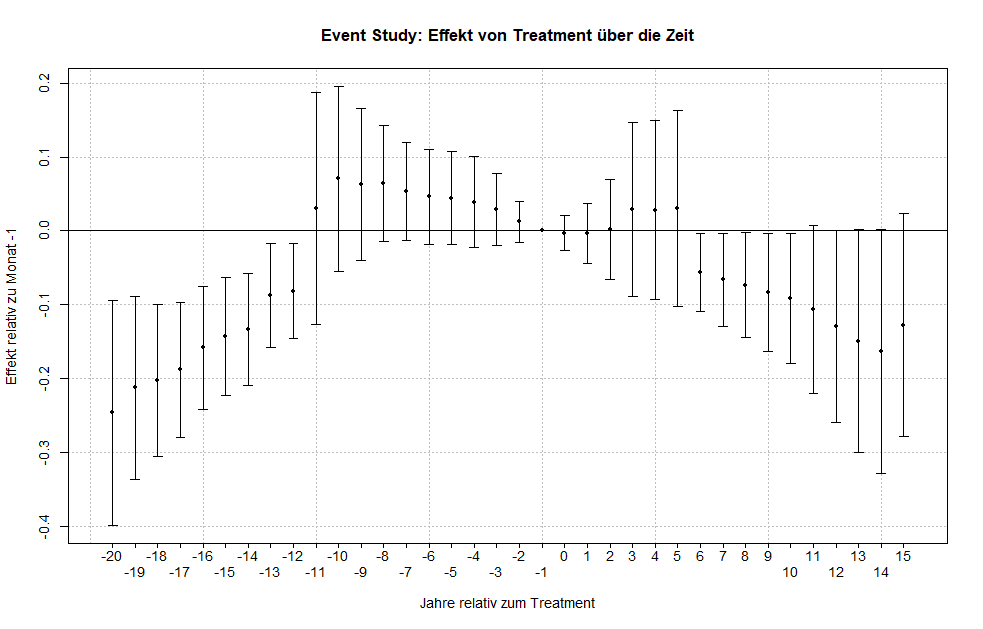
\includegraphics[width=0.8\textwidth]{Eventstudy.png}
\caption{Event study plot showing the estimated coefficients and 95\% confidence intervals over time relative to treatment.}
\label{fig:event_study_plot}
\end{figure}

\vspace{1em}

\section*{5. Interpretation}

The event study results indicate a statistically significant decrease in logged average food prices starting approximately 20 years before the treatment and continuing until shortly after the event, with estimates generally negative and significant in the pre-treatment period.

This pre-trend suggests that treated units were experiencing a downward trend in prices before the treatment, which should be carefully considered when interpreting the causal effect of the treatment.

Post-treatment coefficients fluctuate but generally remain negative with some statistically significant decreases around years 6 to 10 after treatment, suggesting a potential lasting treatment effect.

However, the presence of significant pre-treatment effects signals caution in attributing these changes solely to the treatment without further robustness checks.

\vspace{1em}
\newpage

\section*{6. Conclusion and Recommendations}

While the event study framework provides valuable insight into the temporal dynamics of treatment effects on food prices, the detected pre-treatment trends suggest potential violations of the parallel trends assumption.

We recommend conducting additional robustness tests and considering alternative specifications to strengthen causal inference before making definitive policy recommendations.

\vspace{2em}

\noindent\textit{Prepared by Your Name / Tim Birkert}

\end{document}
